\chapter{Segment Tree}{\label:segment tree}

Segment tree without lazy.
Segment tree with lazy propagation.
Segment tree where common \textbf{combine} is used in update and query.

\medskip
\codecaption{Segment Tree Visualization/Debug}
\begin{lfigure}{resources/dsa-segment-tree-8-nodes.jpg}
{0.6}{0.4} 
\textbf{A segment tree visualization when number of node is power of 2.}
\end{lfigure}

\codecaption{Segment Tree with 11 Nodes}
\begin{lfigure}{resources/dsa-segment-tree-11-nodes.jpg}
    {0.7}{0.3} 
    
    In case of 11 nodes, is it not not $2^k$. The rest of node is distributed evenly below.
\end{lfigure}

\codecaption{Segment Tree Update Visualization}
\begin{lfigure}{resources/dsa-segment-tree-update.jpg}
{0.6}{0.4} 
Function Strucutre: \newline
\verb|update(idx,left,right,START,END,val)|
\verb|query(idx,left,right,START,END)|

\medskip
Main point to note is, \verb|[left,right]| is the range which $idx^{th}$ node represent.

\medskip
To do either operation,we will go from root to leaf. When going down the tree, if the current node is inside the query range \verb|[START,END]| $\Rightarrow$ we will return this node itself. 

\medskip 
Otherwise, we will call for the result of leftsubtree and righttree part seperately. Once the result are available, we will combine them and return it.
\end{lfigure}

\newpage
\begin{fullwidth}
    \begin{figure}
        \caption{Segment Tree Implementation with Array}
        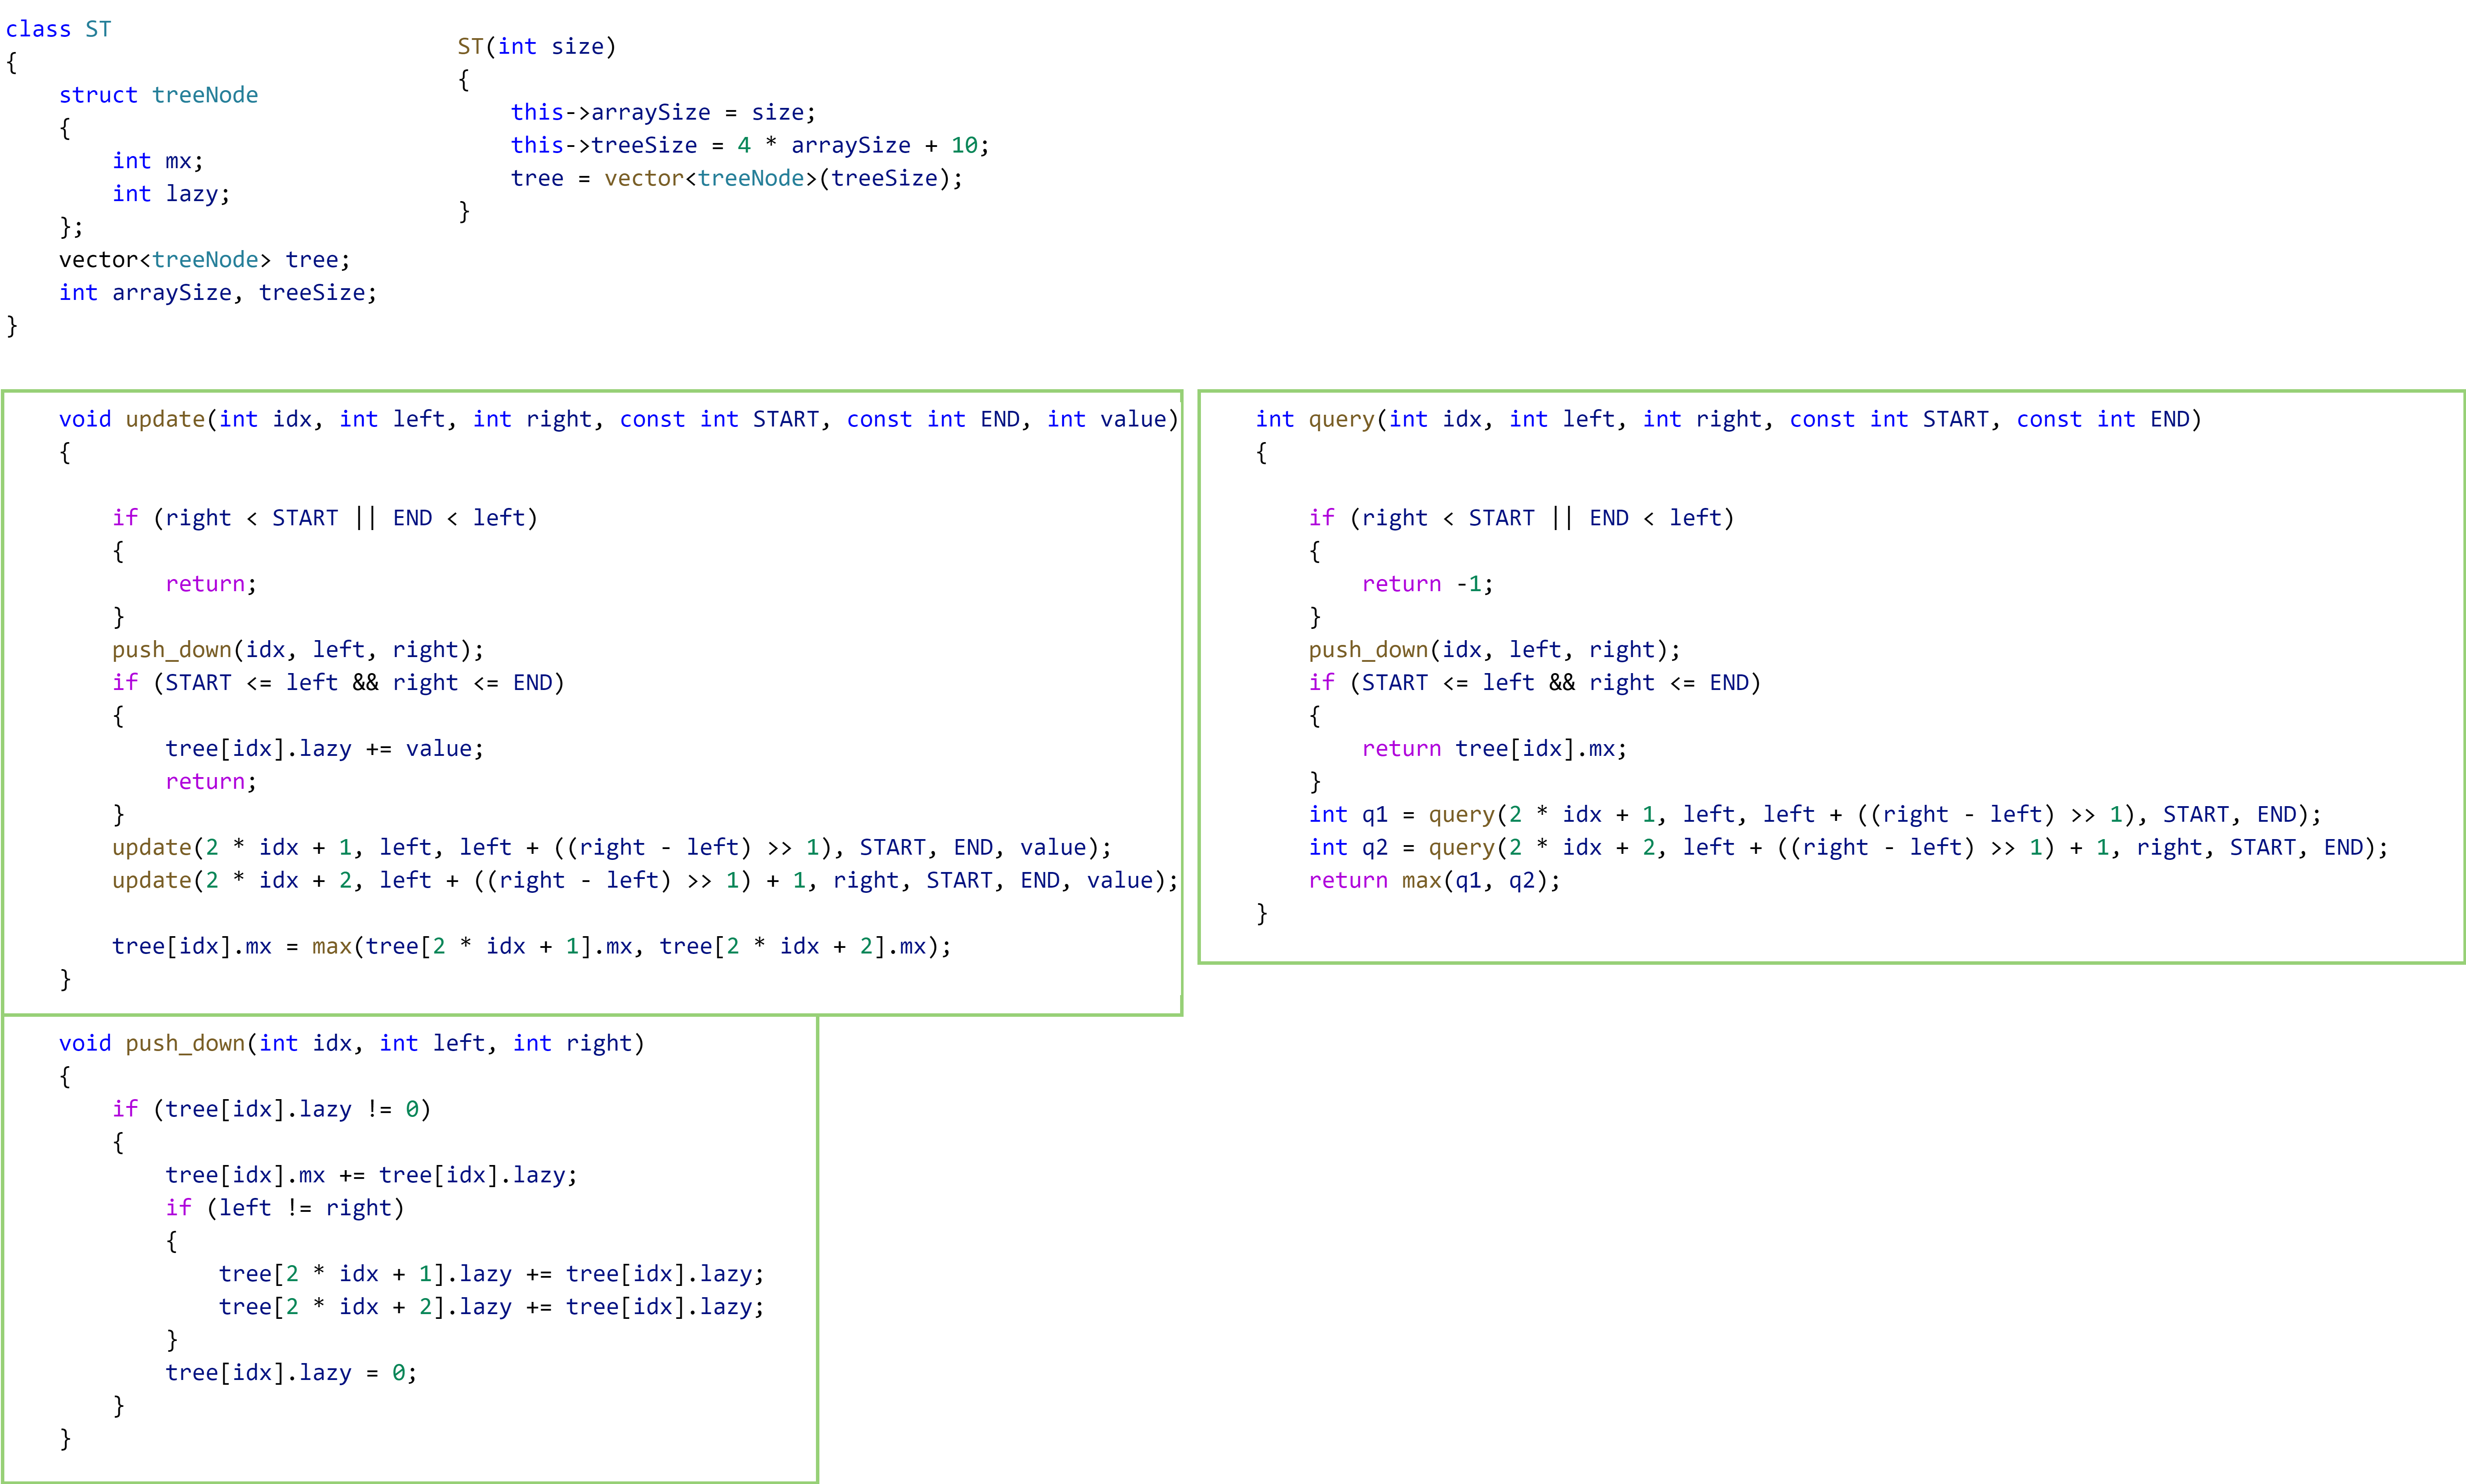
\includegraphics[width=\dimexpr\textwidth+\marginparwidth]{resources/segment-tree-2(idx).png} 
    \end{figure}


    \begin{figure}
        \caption{Segment Tree Implementation With Node}
        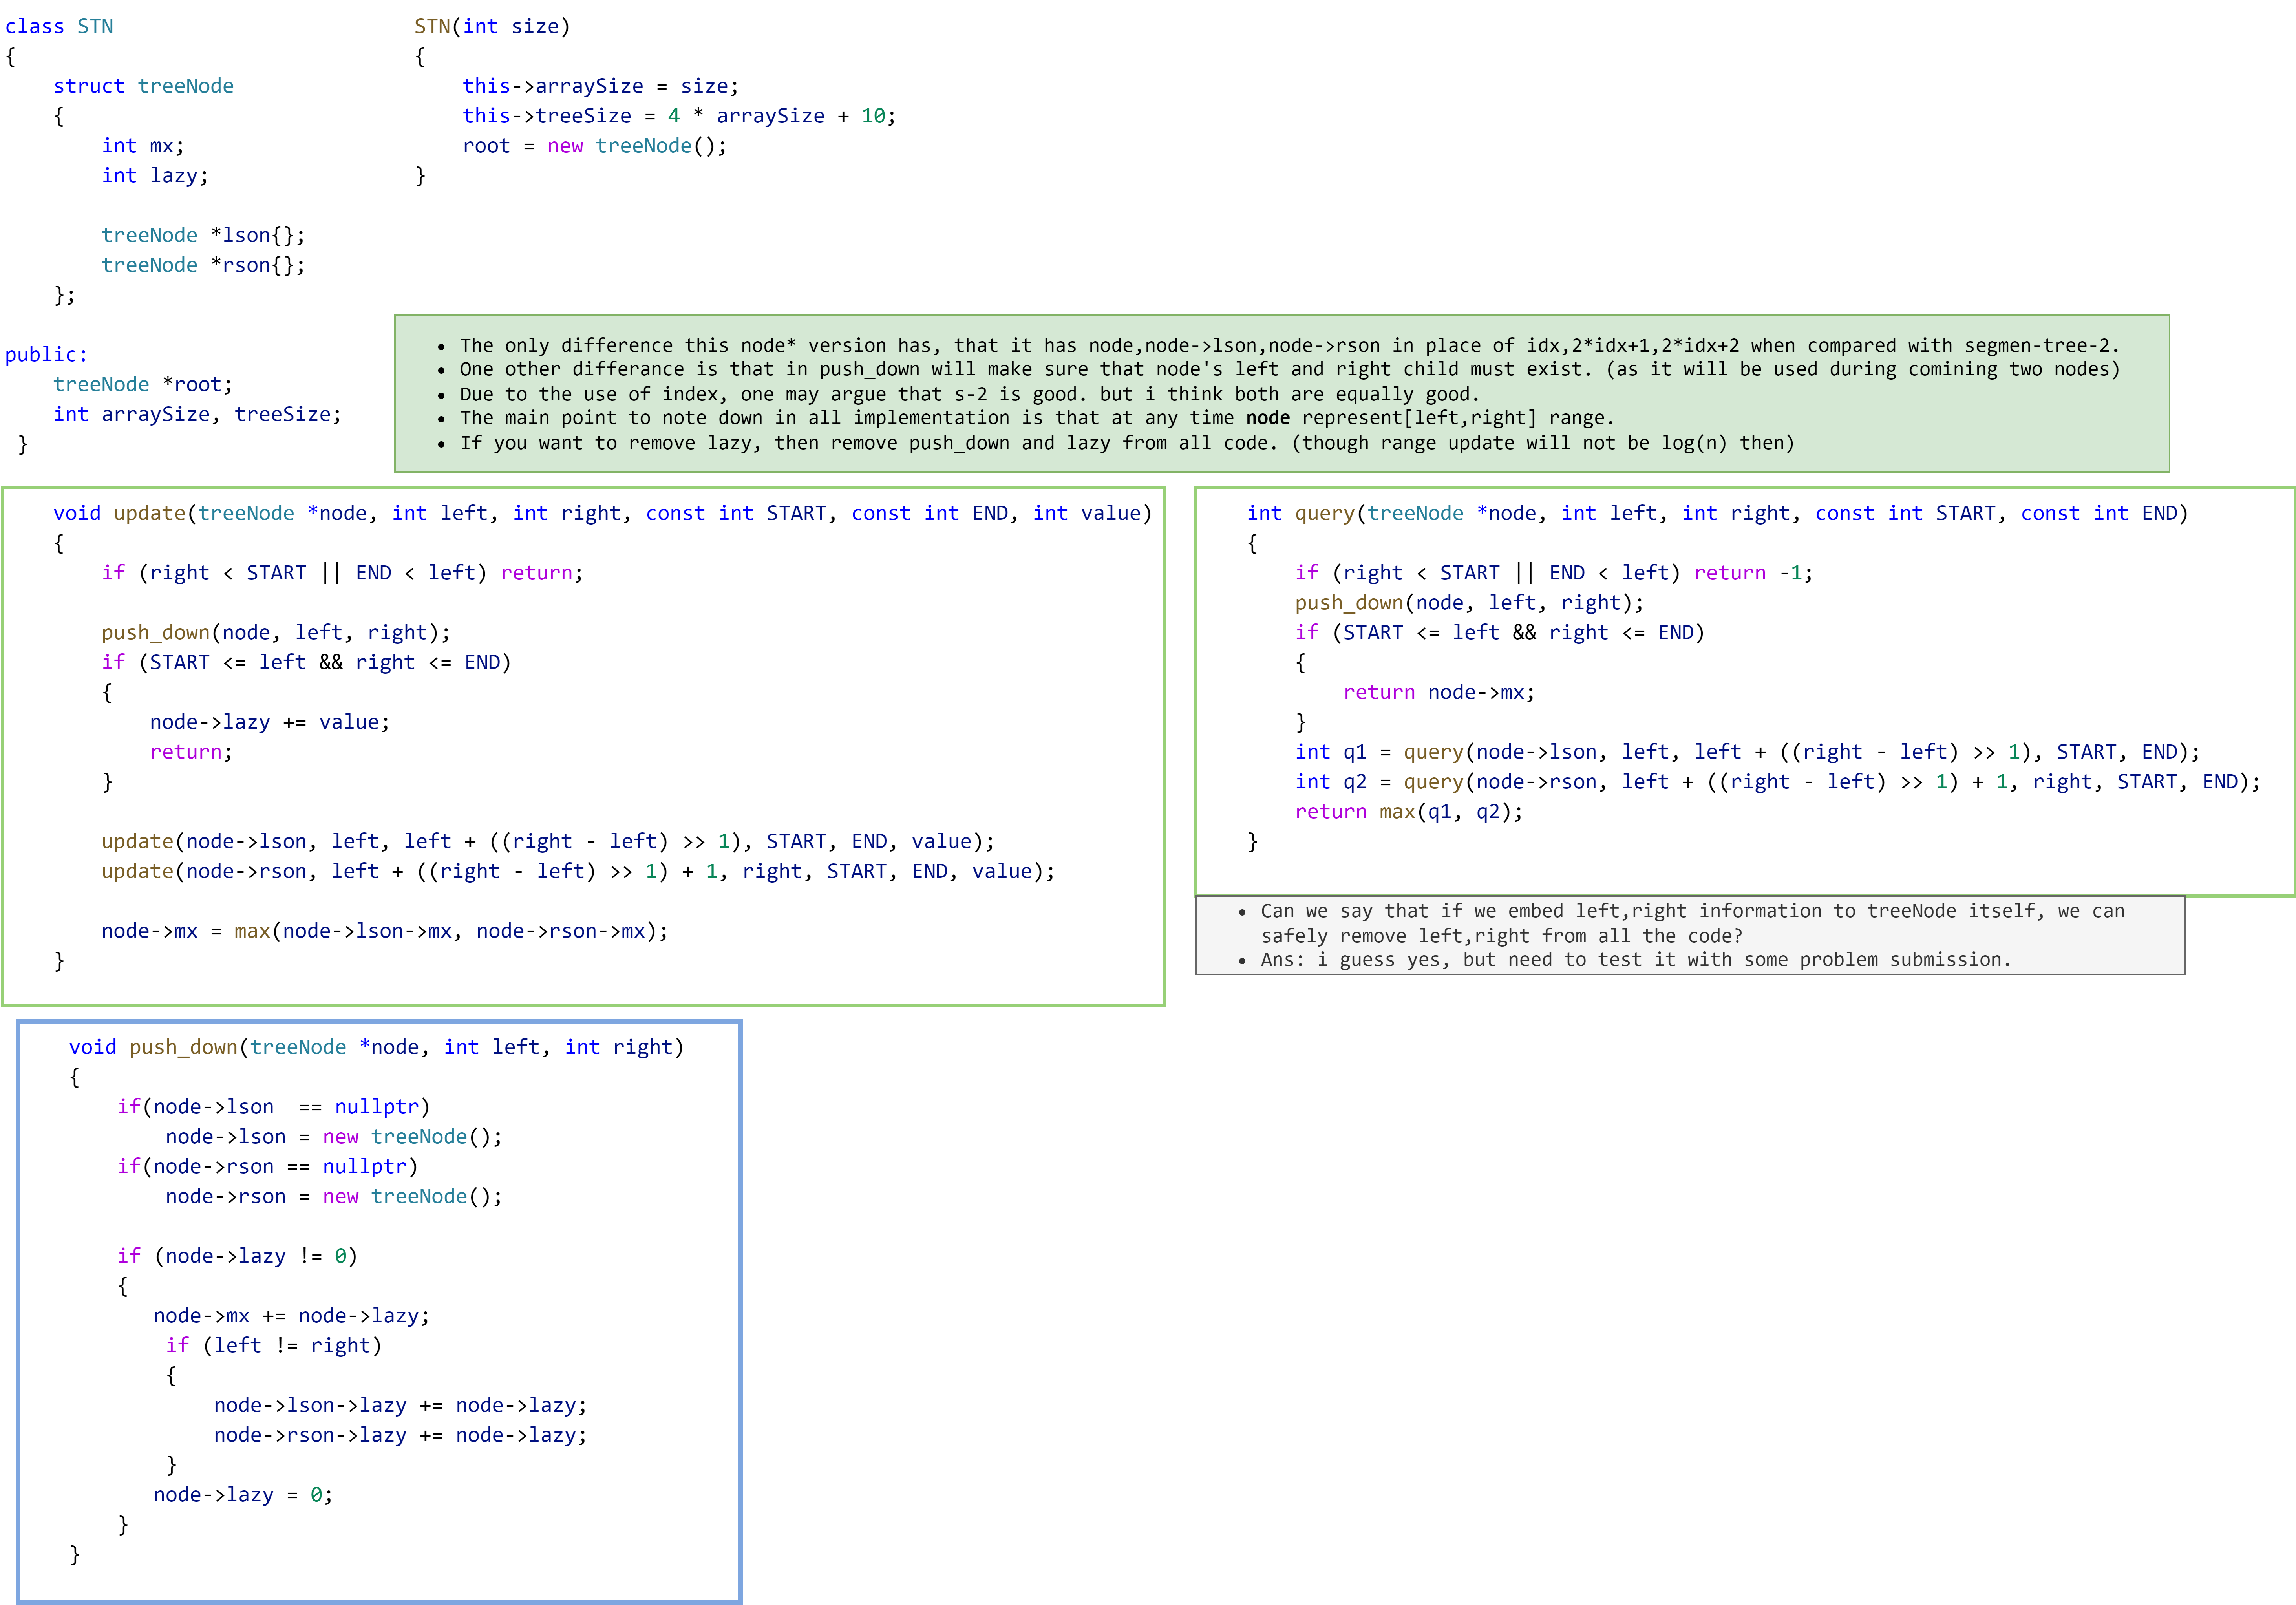
\includegraphics[width=\dimexpr\textwidth+\marginparwidth]{resources/segment-tree-3(node).png}
        
    \end{figure}

    
\end{fullwidth}

{\Large How to Debug Segment Tree?}

Array segment tree can be easiely debugged by printing all node on console. Where for each node you print following info {val,lazy,lson,rson}.
Then you check if corresponsing child nodes where called during update or query ot not.
If not$\Rightarrow$ there is a problem.
You can visualize the tree begin formed as below:


TO-DO: solve a good question , but is solvable in case of issue with above code.

fenwick tree code \href{https://cses.fi/problemset/result/6181195/}{https://cses.fi/problemset/result/6181195/}